\documentclass[conference]{IEEEtran}

\usepackage{epsfig}
\usepackage{fancyvrb}
\usepackage{url}
\usepackage{pifont}

\DefineVerbatimEnvironment%
  {code}{Verbatim}{numbers=left,numbersep=3pt,frame=lines,%
                   xleftmargin=7pt,fontsize=\footnotesize}




\begin{document}


\title{A Component-Based Sensor Network for \\ Environmental Monitoring}

\author{\authorblockN{A. Puder, T. Johnson, K. Sales, M. de Sales}
\authorblockA{San Francisco State University \\
Computer Science Department \\
1600 Holloway Avenue \\
San Francisco, CA 94132 \\
EMail: \{arno$\mid$tlj$\mid$kleber$\mid$msales\}@sfsu.edu}
\and
\authorblockN{D. Robinson}
\authorblockA{San Francisco State University \\
Romberg Tiburon Center \\
3150 Paradise Drive \\
Tiburon, CA 94920 \\
EMail: dhr@sfsu.edu}}


\maketitle
\begin{abstract}
  In this paper we describe a sensor network for environmental
  monitoring based on highly specialized, off-the-shelf sensing
  devices.  Environmental monitoring depends on the reliable
  collection of measurements from remotely deployed sensors and the
  rapid transfer of those measurements to data centers. Typically,
  sensors are deployed in out-of-the-way locations, where physical
  access is limited and connections for telemetry are poor or
  nonexistent. Maintaining the data stream from these sensors places
  demands on human resources, requiring site visits to service the
  sensors and to download data stored on internal memory.  The work
  described in this paper is a collaborative effort between the
  Computer Science Department at San Francisco State University and
  the Romberg Tiburon Center. The result of this collaboration is an
  environmental sensor network deployed in the San Francisco Bay. It
  provides means to program and interrogate sensors at the remote
  field locations and to transmit collected measurements to a remote
  database.
\end{abstract}


\section{Introduction}

A wireless sensor network consists of spatially distributed autonomous
devices using sensors to cooperatively monitor physical or
environmental conditions at different locations \cite{roemer:2004}.
Much research effort is focused on building wireless ad-hoc networks, 
where each sensor node participates in a multi-hop routing algorithm.
One of the earliest examples of a wireless sensor network is the
SmartDust project \cite{smartdust:2001}, where one objective was to
create autonomous sensing and communication in a cubic
millimeter-sized device.  While most wireless sensor networks focus on
small sensing devices such as the SmartDust mote, there exist a wide
variety of off-the-shelf commercially available sensors that are used
by environmental researchers. In contrast to the small sensing
devices, sensors for environmental monitoring are typically on the
order of one to two feet in length, weighing several pounds. Our
focus is on building an end-to-end infrastructure for environmental
monitoring using specialized sensing devices.

Environmental monitoring depends on the reliable collection of
measurements from remotely deployed sensors and the rapid transfer of
those measurements to data centers. Typically, sensors are deployed in
out-of-the-way locations, where physical access is limited and
connections for telemetry are poor or nonexistent. Maintaining the
data stream from these sensors places demands on human resources,
requiring site visits to service the sensors and to download data
stored on internal memory.  Consequently, there is a lag of days to
months between the time the sensors perform the measurements and the
time the measurements become available. Advances in battery life and
anti-fouling technology have extended service cycles for field
sensors, with the unwanted result of further delaying access to
monitoring data.  In addition, the dependence on field site visits to
alter sensor characteristics, such as sampling rate, prevents
adjustments in monitoring strategy in response to rapidly developing
events (e.g. oil spills, harmful algal blooms, among others).

The work described in this paper is a collaborative effort between the
Computer Science Department at San Francisco State University and the
Romberg Tiburon Center (RTC), a research institute focusing on the
understanding of complex marine and estuarine environments. The result
of this collaboration is NetBEAMS (Networked Bay Environmental
Assessment Monitoring System), an environmental sensor network
deployed in the San Francisco Bay. NetBEAMS provides the means to program
and interrogate sensors at remote field locations and to transmit
collected measurements to a database, where the data is rapidly
processed, archived, and made available to potential users in near
real-time. In the following sections we give an overview of the NetBEAMS
architecture and implementation.  Section \ref{SEC_BACKGROUND}
describes a typical environmental sensor used by the RTC. Section
\ref{SEC_DSP} describes our Data Sensor Platform (DSP) that allows us
to efficiently build up an end-to-end environmental sensor network while
Section \ref{SEC_NETBEAMS} describes NetBEAMS. Finally, Section 
\ref{SEC_CONCLUSION} presents our conclusions and future works.


\section{Background}
\label{SEC_BACKGROUND}

Environmental researchers typically use standard, off-the-shelf
sensing devices for their purposes. These sensing devices are at the
opposite end of the size spectrum of miniature sensors such as SmartDust. One such
device is the YSI 6600EDS V2 Sonde \cite{Sonde01}, a water
quality monitoring device that gathers water quality data, and
operates in fresh, sea, or polluted water. Some of the measurements
that the YSI is capable of are conductivity, temperature, chloride,
ammonium, nitrate, turbidity, and chlorophyll.  It is under 55 cm in
length, 8.9 cm in diameter, and weighs approximately 3.18 kg. It
operates at temperatures between -5 to +50 deg C and at depths up to
200 meters.  It uses 8 C-size Alkaline Batteries or External 12 VDC.
Battery life can last up to 75 days depending on sensor configuration.
The Sonde's bulkhead contains multiple pin connectors to support
sensor probes for measuring parameters as shown in Table
\ref{TAB_SONDE_MEASUREMENTS}.

\begin{table}[h]
\caption{\label{TAB_SONDE_MEASUREMENTS} YSI Sonde measurements.}
\centering
\begin{tabular}{|l||l|}
\hline
\multicolumn{1}{|c||}{\textbf{Name}} &
\multicolumn{1}{c|}{\textbf{Description}} \\ \hline \hline
\texttt{Date}    & Year/Month/Day. \\ \hline
\texttt{Time}    & Hour:Minute:Second. \\ \hline
\texttt{Temp}    & Temperature in degrees Celcius. \\ \hline
\texttt{SpCond}  & Specific Description in microSiemens
                   per centimeter. \\ \hline
\texttt{Cond}    & Conductivity in microSiemens per centimeter. \\ \hline
\texttt{Resist}  & Resistivity in Ohms $*$ centimeter. \\ \hline
\texttt{Sal}     & Salinity in parts per thousand. \\ \hline
\texttt{Press}   & Pressure in pounds per square inch relative. \\ \hline
\texttt{Depth}   & Water column in meters. \\ \hline
\texttt{pH}      & pH in standard units. \\ \hline
\texttt{phmV}    & millivolts associated with the pH reading. \\ \hline
\texttt{ODOSat}  & Dissolved oxygen in \% air saturation. \\ \hline
\texttt{ODOConc} & Dissolved oxygen in mg/L. \\ \hline
\texttt{Turbid}  & Turbidity in nephelometric turbidity units. \\ \hline
\texttt{Battery} & Total Volts remaining in batteries.  \\ \hline
\end{tabular}
\end{table}


Each probe may have multiple sensors.  A computer can interface with
the Sonde via RS-232C or SDI-12. The Sonde can be configured to
collect data samples in discrete or unnattended mode.  Discrete mode
is normally performed while a technician manages the Sonde during the
sampling process. In this mode, the Sonde is connected via 650
MDS Display/Logger or a serial cable connected to a PC, where the sampling
frequency is usually set to a high frequency. In contrast, Unattended
mode is performed when the Sonde is deployed offshore or in a
remote body of water, where the sampling frequency is usually set for a
longer period of time (i.e. 5 - 15 min). Assuming a 5 min sampling
frequency, the Sonde produces 267 KB of data per day.
In order to be configured,
the Sonde offers a set of menus that can be accessed through a terminal session
over RS232. In this way, the Sonde can be configured to
start logging data to an internal file. In order to view the data as it's
being captured, the option to show live data is chosen and the data can then be 
seen via a serial terminal session at each interval.

We provide these details to show that sensing devices such as the YSI
are highly specialized devices with a unit price of several thousand
dollars. These sensors are usually sparsely deployed in remote
locations that not only make their maintenance difficult, but also
access to their measurements difficult.  Typically, the sensors are autonomous
in the sense that they can run for a certain amount of time on battery power and
store the measurement data in internal memory. Only when the sensors
are serviced, the measurement data, which was collected since the last
servicing, is uploaded to a portable storage device. From there, the
data can be uploaded to server. This manual procedure to retrieve
sensor data is not only error prone, but the results greatly differ
between the time the sensor performs the measurement and when
it becomes available for further processing. For many applications,
however, it would be beneficial to have near-realtime access to the
sensor measurements. We identify the following requirements that an
end-to-end infrastructure supporting devices such as the YSI should
offer:

\begin{itemize}
\item Allow near-realtime access to sensor measurements;
\item Allow remote servicing that include changing of configuration
  parameters as well as software upgrades;
\item Support cost-effective long distance communication link;
\item Can be deployed in remote locations in unprotected outdoor
  conditions.
\end{itemize}

In the next section, we describe a software architecture that provides
a foundation to fulfill these requirements.


\section{Data Sensor Platform}
\label{SEC_DSP}

Sensor networks, especially environmental sensors, are normally
deployed over a geographically wide area, where the communication
infrastructure is not always reliable or, at least, not coutinuously
available. As the sensor network grows in size and complexity, 
scalability, reliability and maintainability become critical issues.
For instance, additional components might be added to the network, sensor
configuration might be altered, or new versions of components might have to be
deployed. As a consequence, the sensor network must be able to support such
adjustments without significant overhead for maintainers.  From a system
development and integration point of view, interfaces among components
and between components and the network should be simple. As a result, complex
interaction can be constructed on top of these simple interfaces. In
the following subsections, we discuss how our proposed architecture addresses
those issues.

\subsection{Architecture}

NetBEAMS's architecture is based on a micro-kernel approach. The core
functionality is limited to a minimum and all extra services are built
as plug-and-play modules on top of the micro-kernel. With the help of
this approach, we can keep the basic infrastructure compact while
allowing customization via special-purpose modules. In our terminology,
we call the basic foundation the \emph{Data Sensor Platform}
(DSP). The scope of the DSP is one address space of an execution
platform and a sensor network is built from several DSPs that are linked
with each other.

Figure \ref{FIG_DSP} depicts the basic architecture of the DSP. We
refer to the plug-and-play modules as DSP Components. DSP Components
are self-contained modules that can be added and removed to a DSP
installation at runtime. The basic communication unit within a DSP
is a message. DSP Components can exchange messages of different types.
Actually, all interactions between DSP Components are implemented
through messages yielding a simple but powerful communication
structure. Moreover, we distinguish between \emph{Data Producers} (DP) and
\emph{Data Consumers} (DC) within the scope of a DSP. DP and DC can be
seen as roles that a DSP Component may have, as it may also 
act in the role of DC and DP at the same time. Messages
in DSPs are routed based on rules, which can be configured statically
or dynamically. Rules for routing messages can be based on different
information such as producers or consumers of the message, the message
itself, or specific configuration parameters provided externally.

\begin{figure}
\centering
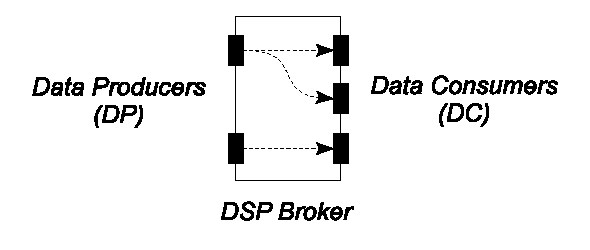
\epsfig{file=dsp, width=7cm}
\caption{\label{FIG_DSP} Data Sensor Platform (DSP).}
\end{figure}

The DSP is responsible for routing messages between DPs and DCs. It is
important to note that this routing only happens within a
DSP. Following the paradigm of a micro-kernel approach, the DSP has no
notion of remote communication or sensor-specific details. All this
knowledge is embodied in special purpose DSP Components.

\subsection{DSP Components}

A DSP Component encapsulates a particular functionality. We
distinguish between those components that produce data (DP) and those
that consume data (DC). An example for a DSP Component acting in the
role of a DP is a module that interfaces with a physical sensor. Such
a module reads data from the sensor and converts the data into a
message that is forwarded to the DSP. Because this module generates
data with respect to the DSP, it is a data producer. An example for a
data consumer is a converter module that converts the internal,
DSP-specific data format to a format suitable for consumption by
external applications. One such common format used in the domain of
environmental monitoring is OpenDAP \cite{opendap01}.  Since the
converter module accepts messages from the DSP, it acts in the role of
a data consumer. Finally, a DSP Component implementing persistence is
an example of a module that acts in the roles of both data producer
and consumer, since it accepts messages from the DSP and stores them in a
database. Furthermore, it may act as a data producer by resending previously
stored messages at a later time.

All DSP Components need to implement the following Java interface:

\begin{code}
interface DSPComponent
{
   public String getComponentType();
   public void initComponent(String     id, 
                             DSPContext context);
   public void startComponent();
   public void stopComponent();
   public void deliver(DSPMessage msg);
   // ...
}
\end{code}

By implementing the above Java interface, the resulting code
effectively becomes a DSP Component that can be deployed on a DSP at
runtime. A component is identified by its type (line 3). Only one
component of a certain type per DSP is permissible. A type identifier
must be unique across all DSP Components in a DSP. Upon deploying a
component, an initialization function is called (line 4). Once a
component is initialized, it may be started (line 6) and stopped (line
7) multiple times. Whenever the DSP wishes to pass a message (that was
generated by some DP), it invokes the \texttt{deliver()} method (line
8). A DP can send messages via a \texttt{DSPContext} object that was
passed to the DP during initialization.

\subsection{Message Structure}

Message passing is the main paradigm for exchanging information within
a DSP. After producing data, a DP wraps that data in the body
of a message, so that DC components can receive the message and
consume the data contained in the message's body. When it comes to passing
messages to a remote DSP instance, messages are serialized in XML
\cite{xml2000} and automatically deserialized for DCs located in the
remote DSP. In order to serialize and deserialize DSP messages, the
DSP infrastructure uses the XML Schema standard \cite{xml-schema2004}
to generate and validate the DSP message. Figure \ref{FIG_DSP_MESSAGE}
defines the structure of a general DSP message.

\begin{figure}[!htb]
 \centering
 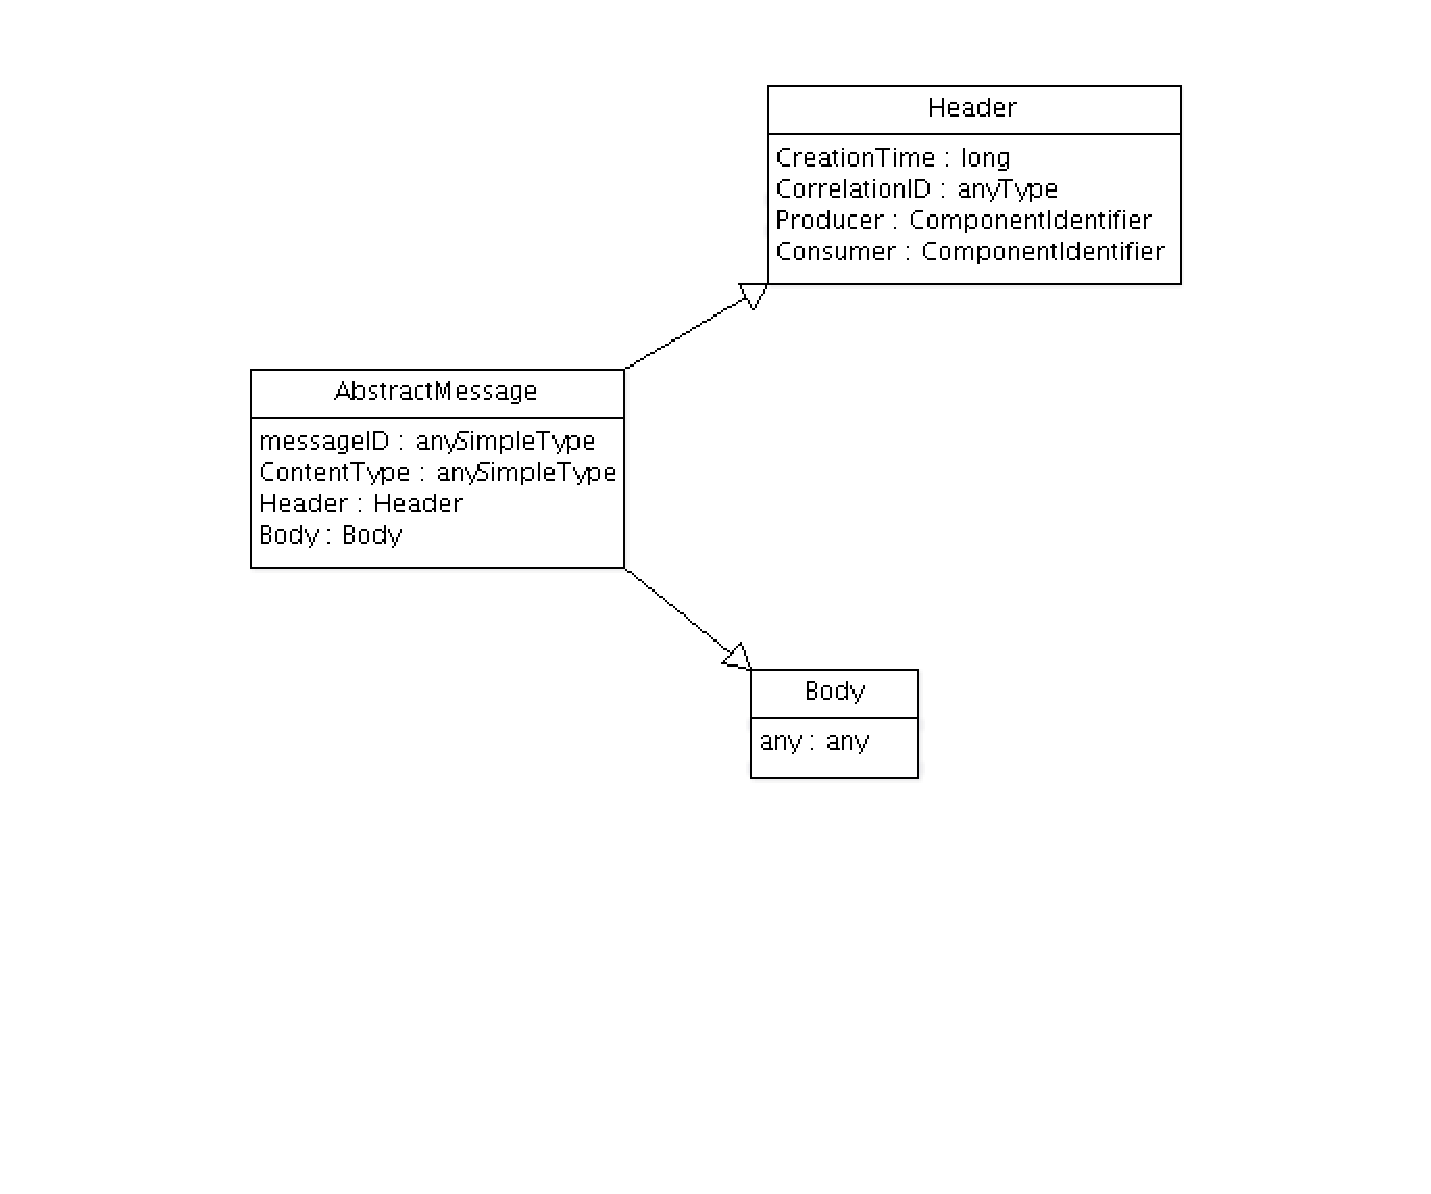
\epsfig{file=AbstractMessage, width=9cm, height=4cm}
 \caption{\label{FIG_DSP_MESSAGE} Structure of a DSP message.}
\end{figure}

The basic message structure is defined by an \texttt{AbstractMessage}
type, whose structure serves as a base schema for all different types
of messages. Any message will contain two basic attributes:
\texttt{messageID} and \texttt{ContentType}.  The former uniquely
identifies a message and the latter the data in the body of the
message. Complementary identification information, such as the message
producer and consumer, is located in the header of the message and 
is defined by the schema type \texttt{ComponentIdentifier}. A
\texttt{ComponentIdentifier} carries out information about the
component name and its physical host address.  Finally, the body of
the message represents the payload and may contain any data type
defined by the component developer.

XML schema is the de-facto standard to bind and validate XML
data to its type. Within the DSP we use an XML
data binding technology \cite{xml-dbind} called JAXB \cite{xml-jaxb}.
It is used to generate a type safe API for handling in-memory object
graphs from the XML instances of DSP Messages and the content of its
data payload. Moreover, taking advantage of the data type polymorphism
of XML schema data types, we defined different categories of messages in order to
reflect the nature of the message content. Among those categories are
query and update messages, where the former is used for configuring various
properties supported by DSP Components, and the latter is used for measurement
messages that actually contain sensor readings.

The payload of a message is itself described via an XML schema in
order to integrate it seemingly with the general message structure. By these
means, a developer of a DSP Component can define a schema that represents the
type of payload processed by that component. An example illustrating a DSP
message is given when we discuss the YSI Sonde Component.

\subsection{DSP Broker and Matcher}

The \emph{broker} is responsible for routing the message to one or
several DCs. It distinguishes between local and remote destinations:

\begin{itemize}
\item Local delivery of messages: it uses local object reference to
  deliver the DSP message.
\item Remote delivery of messages: it uses a DSP Component marked as a
  gateway to handle remote message delivery.
\end{itemize}

The broker can deliver messages concurrently and asynchronously. It
sets any additional message header information necessary for proper
routing. The broker does not make any routing decisions. It delegates
this responsibility to the \emph{matcher}. The matcher is responsible
for matching messages sent by a DP and routes it to one or more DCs.
This decision is based on a set of routing rules (see Figure
\ref{FIG_MATCHER_RULE}) which can be statically or dynamically
configured.

\begin{figure}[!htb]
 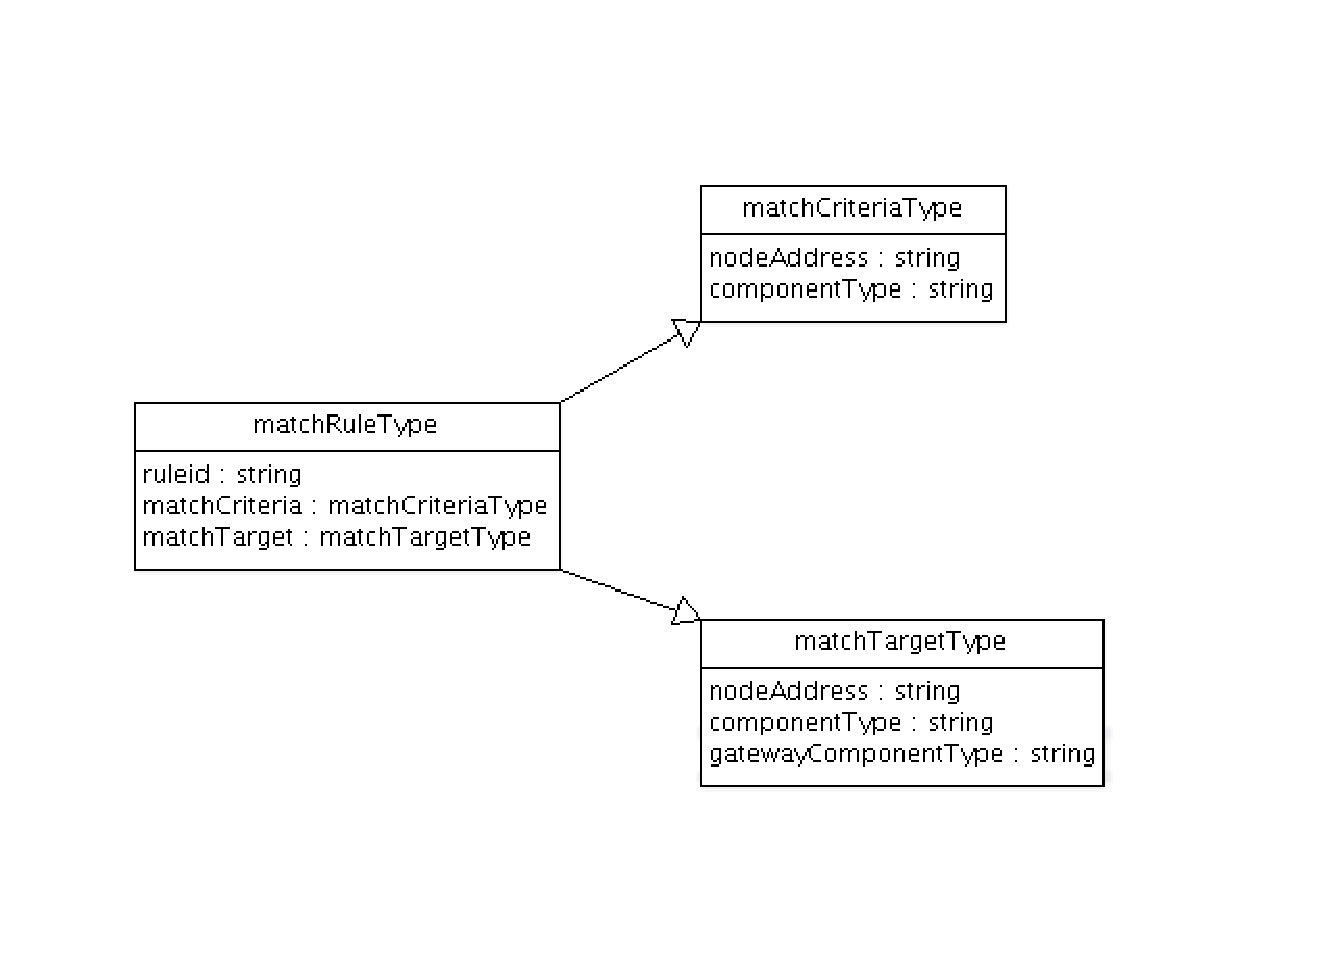
\epsfig{file=MatcherRule, width=9cm, height=4cm}
 \caption{\label{FIG_MATCHER_RULE} Definition of Matcher Rule.}
\end{figure}

\begin{itemize}
\item The \emph{match criteria} defines the name of the component type
  of the producer and its physical location (IP address).
\item The \emph{match target} defines the name of the component type
  of the consumer, and optionally defines a gateway component.
\end{itemize}

The matcher's main purpose is to achieve a loose coupling between
DCs and DPs. DPs may create messages without specifying a specific
destination DC. Once the message is sent through the DSP, the matcher will
determine which DCs should receive the message. Note that, a DP can
still specify a DC for its message. In this case, the matcher includes
this DC in a list of DCs to receive the message.



\section{NetBEAMS}
\label{SEC_NETBEAMS}

\begin{figure*} 
\centering
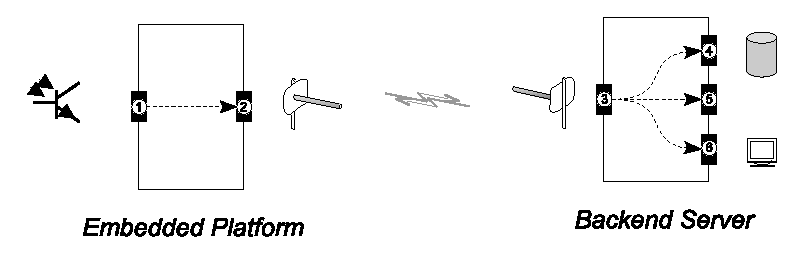
\epsfig{file=netbeams, width=14cm}
\caption{\label{FIG_NETBEAMS} NetBEAMS architecture.}
\end{figure*}

In the following subsection, we present a practical application of the DSP
introduced in the previous section. Our environmental sensor network
is dubbed NetBEAMS (Networked Bay Environmental Assessment Monitoring
System) and allows access to sensor equipment deployed throughout the
San Francisco Bay Area. This end-to-end system is a ready-to-use
turnkey solution that is adaptable to a wide variety of sensor types
and requires no programming expertise to operate. Configuration of the
system will be possible when the sensor is deployed in the field via a
web-based interface, eliminating the need for extra site visits by
technicians between service cycles to change system characteristics
such as the sampling rate.  We present the NetBEAMS infrastructure by
discussing its hardware and software components.


\subsection{Hardware}

Figure \ref{FIG_NETBEAMS} provides an end-to-end overview of the
NetBEAMS architecture. NetBEAMS is built using multiple installations
of the DSP and by providing special purpose components for the various
tasks. One DSP installation is collocated with each sensor and an
additional DSP is running on the backend server. Because of the remote
locations where each individual sensor is deployed in the field and
the sparse density of the network, the resulting topology is a tree
structure of depth 1.

NetBEAMS supports an environmental sensor such as the YSI Sonde,
introduced in Section \ref{SEC_BACKGROUND}. In order to access its
sensor readings, we collocate it with an off-the-shelf embedded
computing platform called Gumstix \cite{gumstix01} (far left in Figure
\ref{FIG_NETBEAMS}).  The Gumstix is an ARM-based single board computer and comes in
various configurations.  A typical Gumstix configuration
consists of a motherboard and one or more expansion boards that
connect to the motherboard via on-board buses.  The motherboards draw
less than 250 mA @4V at 400 MHz and less than 50 mA while idling,
waiting for input.

The Gumstix runs Linux 2.6 with the BusyBox utilities, and uses the
OpenEmbedded cross-compile build environment to provide a complete
Linux environment and a large range of Linux applications for the ARM
architecture.  We use the JamVM \cite{jamvm01} implementation of Sun
Microsystem's virtual machine in order to run the DSP. The Gumstix
communicates with the YSI Sonde via an RS232 serial port using a
null-modem cable, since both the Sonde and the Gumstix are DTE devices.
%The serial port configuration is:

%\begin{table}[!htb]
%\caption{\label{tab:RS232_Config}RS232 Serial Port Configuration}
%\centering
%\begin{tabular}{l l}
%\hline
%Baud Rate&9600\\
%Data Bit&8\\
%Parity&None\\
%Handshake&None\\
%\hline
%\end{tabular}
%\end{table}


%\begin{table}
%\caption{\label{TAB_RS232_Pinout}RS232 Serial Pinout}
%\centering
%\begin{tabular} {|l|l|l|}
%\hline
%Wire Color	&Pin Description        &DB-9\\ 
%\hline
%Yellow 		&RS232 TX    &2\\
%Orange		&RS232 RX    &3\\  
%Green  		&Alarm       &----\\ 
%Grey			&RTS         &----\\
%Blue  		&CTS         &----\\
%Red			&+ 12V DC    &9\\
%Black			&GND         &5\\  
%Purple		&SDI-12      &----\\ 
%Bare			&Shield      &----\\
%\hline
%\end{tabular}
%\end{table}
 

We make use of the cellular phone network to establish a communication
link with the backend server. The cellular phone network has the
advantages of reaching well beyond telemetry options such as wireless
networks and being a significantly lower cost solution than satellite
communications. We make use of the Huawei E220, which is a USB
modem that supports HSDPA, UMTS, and EDGE packet data services at
maximum transmission rates of 3.6Mbps, 384kbps, and 236.8kbps
respectively.  HSDPA and UMTS operate at 2100MHz while GSM, GPRS, and
EDGE operate at 900, 1800, and 1900MHz. The modem connects to the
Gumstix motherboard via a mini USB interface (supporting USB 2.0). In this
way, the Gumstix communicates with the modem using the PPP protocol and
accesses the cellular network using a data plan from AT\&T.



\subsection{DSP Implementation}

The DSP is implemented in Java and serves as a container environment where 
DSP Components execute. Due to its micro-kernel, modular and dynamic characteristics, 
the current DSP implementation uses OSGi \cite{osgi} as a deployment and execution 
infrastucture. One important DSP requirement is to impose on DSP Components minimal 
dependency on the DSP itself and no depency on OSGi. To this extent, all DSP resources
accessible to DSP Components are specified by \texttt{DSPContext} interface.
The DSP also uses messages to communicate with DSP Components. It has a special adapter
that acts like a \texttt{DSPComponent}. Therefore, configuring the DSP is no different from configuring
a DSP Component.

DSP Compoments are deployed as OSGi bundles. OSGi defines bundles life-cycle and
runtime upgrade mechanism. DSP uses these capabilities to allow remote deployment 
(bundles with DSP Components are transmitted as message to the DSP Component Adaptor) 
and activation/deactivation of DSP Components. 

Our implementation of the DSP is based on the Open-Source
implementation of OSGi called Knopflerfish \cite{knopflerfish01}.
Since Sun Microsystems does not support its JDK for the Gumstix, we
use JamVM \cite{jamvm01} as the Java virtual machine implementation
and the GNU Classpath \cite{classpath01} project for the runtime libraries. In
the following sections, we provide further details of some of the DSP
Components that we have implemented as part of the NetBEAMS project.

\subsection{YSI Sonde Component}

On the far left of Figure \ref{FIG_NETBEAMS} is the actual sensor; in
our case, the aforementioned YSI Sonde. The YSI Sonde DP \ding{192}
uses the RS232 standard to read the physical measurements from the
device over a serial port.  This component converts the physical
measurements into a DSP-specific message. Figure
\ref{FIG_DSP_YSI_DATA} depicts the YSI Sonde's specific message format, 
which includes each measurement data point, described in Table
\ref{TAB_SONDE_MEASUREMENTS}.

\begin{figure}[!htb]
\centering
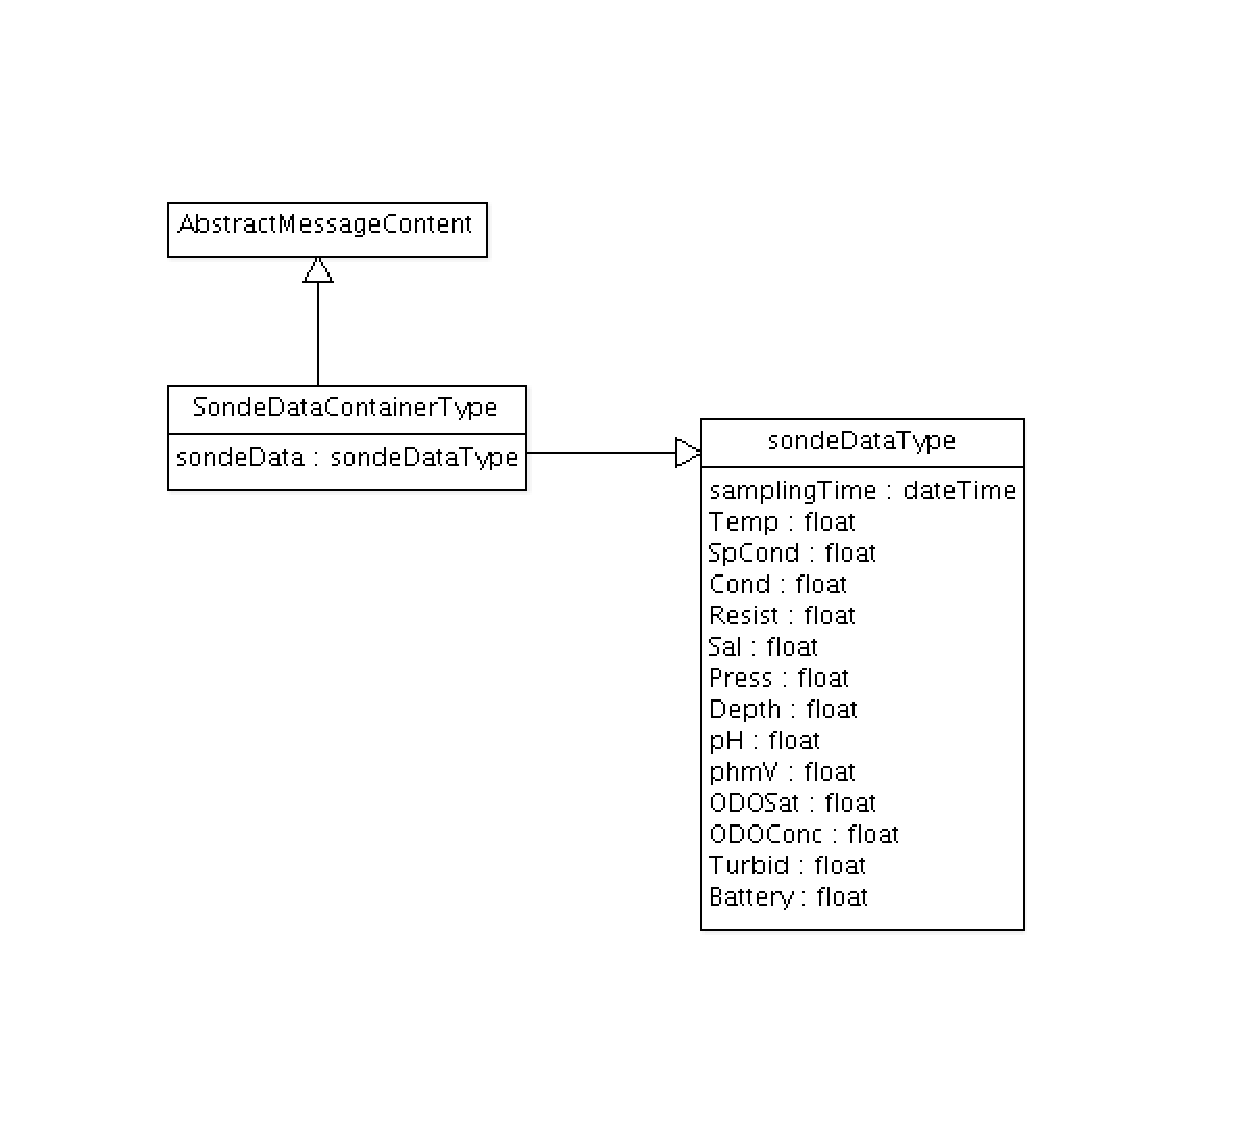
\epsfig{file=YSI_Message_Format, width=9cm, height=5cm}
\caption{\label{FIG_DSP_YSI_DATA} YSI message format.}
\end{figure}

The \texttt{SondeDataContainerType} defines the payload of messages generated
by the YSI Sonde DP. As all DSP messages, it is derived from the
\texttt{AbstractMessageContent}. The payload mainly consists of the
\texttt{SondeDataType} that defines all the sensor data that the YSI Sonde is
capable of producing. The YSI Sonde DP uses the RS232 to query the
physical device for its data in regular intervals. The measurements
are then converted into a DSP message and forwarded to the DSP Broker,
from which they are forwarded to the remote communication component
described in the next section.  The YSI Sonde DP can also be
configured via special Update DSP messages, to direct the Sonde to change its
sampling frequency.  These property messages originate from a web
management interface (component \ding{197} in Figure \ref{FIG_NETBEAMS}).


\subsection{Remote Communication}

All messages sent by the YSI Sonde DP need to be uploaded to a remote
database. Since the DSP itself can only handle communication within
its local DPs and DCs, we have created a matching pair of DC and DP
that can handle remote communication (components \ding{193} and \ding{194} in Figure
\ref{FIG_NETBEAMS}). As explained earlier, we make use of the cellular
phone network to upload sensor data to a remote backend server. While
the cellular phone network has sufficient coverage for more
environmental sensor networks, it is not cost effective to keep a data
link permanently open. The remote communication components can be
configured to upload buffered sensor data only in certain time
intervals. With this in mind, DSP Messages are transported via HTTP
\cite{RFC2068}. In this way, the matching DP/DC pair for remote communication
has the following properties:

\begin{itemize}
\item DSP Wire Transport Client: takes a collection of DSP messages
  and transmit them via HTTP. As a non-functional requirement, the
  interval in which this component will transmit messages to other
  components can be configured via the management interface;
\item DSP Wire Transport Server: is an HTTP server that receives the
  collection of DSP messages sent by the client, and piggy backs any
  messages destined for the remote client that may have queued up in
  the meantime.
\end{itemize}

The HTTP request and response are used to upload and download any
messages that have been queued at the respective end of the
communication link. The client and server components are capable of
buffering messages until they are sent to the remote destination
during the next communication cycle. Once messages have been
transported to their final destinations, they are unmarshalled and
passed on to the local DSP Broker for further dispatching. In this
regard, the client and server components are completely symmetrical. Messages
are dispatched with the help of the matcher to their final destinations.


\subsection{Web Management}

One of the NetBEAMS goals is to easily configure the sensor
network without programming skills. Technicians should be able to
change configuration parameters of various DSP Components via an
easy-to-use web interface. With regards to the NetBEAMS specific
components discussed in earlier sections, these configuration
parameters are, for example, the sampling frequency of the YSI Sonde DP
and the upload frequency of the the wire transport DC.

This configuration is performed by a special DSP Component that
offers a web interface through which a technician can define the
configuration parameters (component \ding{197} in Figure
\ref{FIG_NETBEAMS}). The web management component first queries the remote
component to get a list of configuration parameters. Once the remote
component sends a reply, a user interface is automatically built up
to allow the entry of user defined values. When those values are
submitted, an update message is sent back to the remote component that
will then change the appropriate configuration parameters.

The user interface offered by the web management component is
asynchronous in the sense that there might be a time lag between a
request and a response. This has to do with the fact that the remote
DSP will only establish a communication link at certain time intervals
during which the query and update messages will be forwarded. Apart
from component configuration, the web management component is also
capable to remotely start, stop, and re-deploy new versions of DSP
Components.

\section{Conclusions}
\label{SEC_CONCLUSION}

%The California coastal region is populated by a vast number of
%remotely deployed sensors that monitor environmental conditions
%ranging from weather to water quality to ocean surface currents.
%These sensors are operated by data providers, including resource
%management groups, research scientists, municipalities, state and
%federal agencies, who could use near real-time data streams to inform
%decisions that impact public health, public safety, and the protection
%of resources. Success of these efforts, whether small scale or a large
%integrated network, depends on the first step in the data management
%process: reliably obtaining data in near real-time from remotely
%located sensors.  This step can be the weak link in the data
%management pathway when telemetry options are unreliable.  The
%availability of a plug-and-play computing platform designed to
%communicate with a variety of sensor types would stabilize data
%streams with poor telemetry and allowing expansion of sensor coverage
%into regions not presently served.

In this paper, we introduce a practical application of a sensor network
in the domain of environmental monitoring. We have built an
environmental sensor network in the San Francisco Bay using highly
specialized, off-the-shelf water quality sensors. The resulting
infrastructure enables near-realtime access to sensor data collected
from remote locations. Our end-to-end solution, furthermore, allows
configuration and management of remotely deployed sensors. In this sense, the
key to our infrastructure is the DSP, a micro-kernel plug-and-play
architecture that can flexibly be configured to specific needs through
special purpose components. We plan to use the Gumstix's processing
power to pre-process data intensive sensors such as the HF Radar to
reduce the data volume.


Furthermore, our work improves upon existing technologies in earlier sensor network implementations.
Many sensor networks use PIC microcontrollers \cite{Pic01} and specialized operating systems
such as TinyOS \cite{tinyos01}. However, PICs are usually too buggy,
requiring non-standard operating systems \cite{Martinez04}. Likewise, TinyOS exhibits limited 
constraints on storage, restricting any complex processing of sensor data
that can be performed \cite{Martinez04}. OSGi has been used in other sensor network
projects \cite{Mueller07, Baude07}. Although some OSGi sensor networks also include remote 
communication capabilities \cite{Rellermeyer}, our DSP is designed to support asynchronous 
communication in loosely coupled networks. The NetBEAMS infrastructure, as
described in the paper, is available as an Open-Source project and can be 
viewed in operation at \texttt{www.netbeams.org}.



\bibliography{lit}
\bibliographystyle{plain}


\end{document}
